% 论文插图代码片段示例
% 使用前请确认 thesis.tex 已引入 graphicx、float、subcaption 宏包

% 单张界面图示例：首页
\begin{figure}[H]
  \centering
  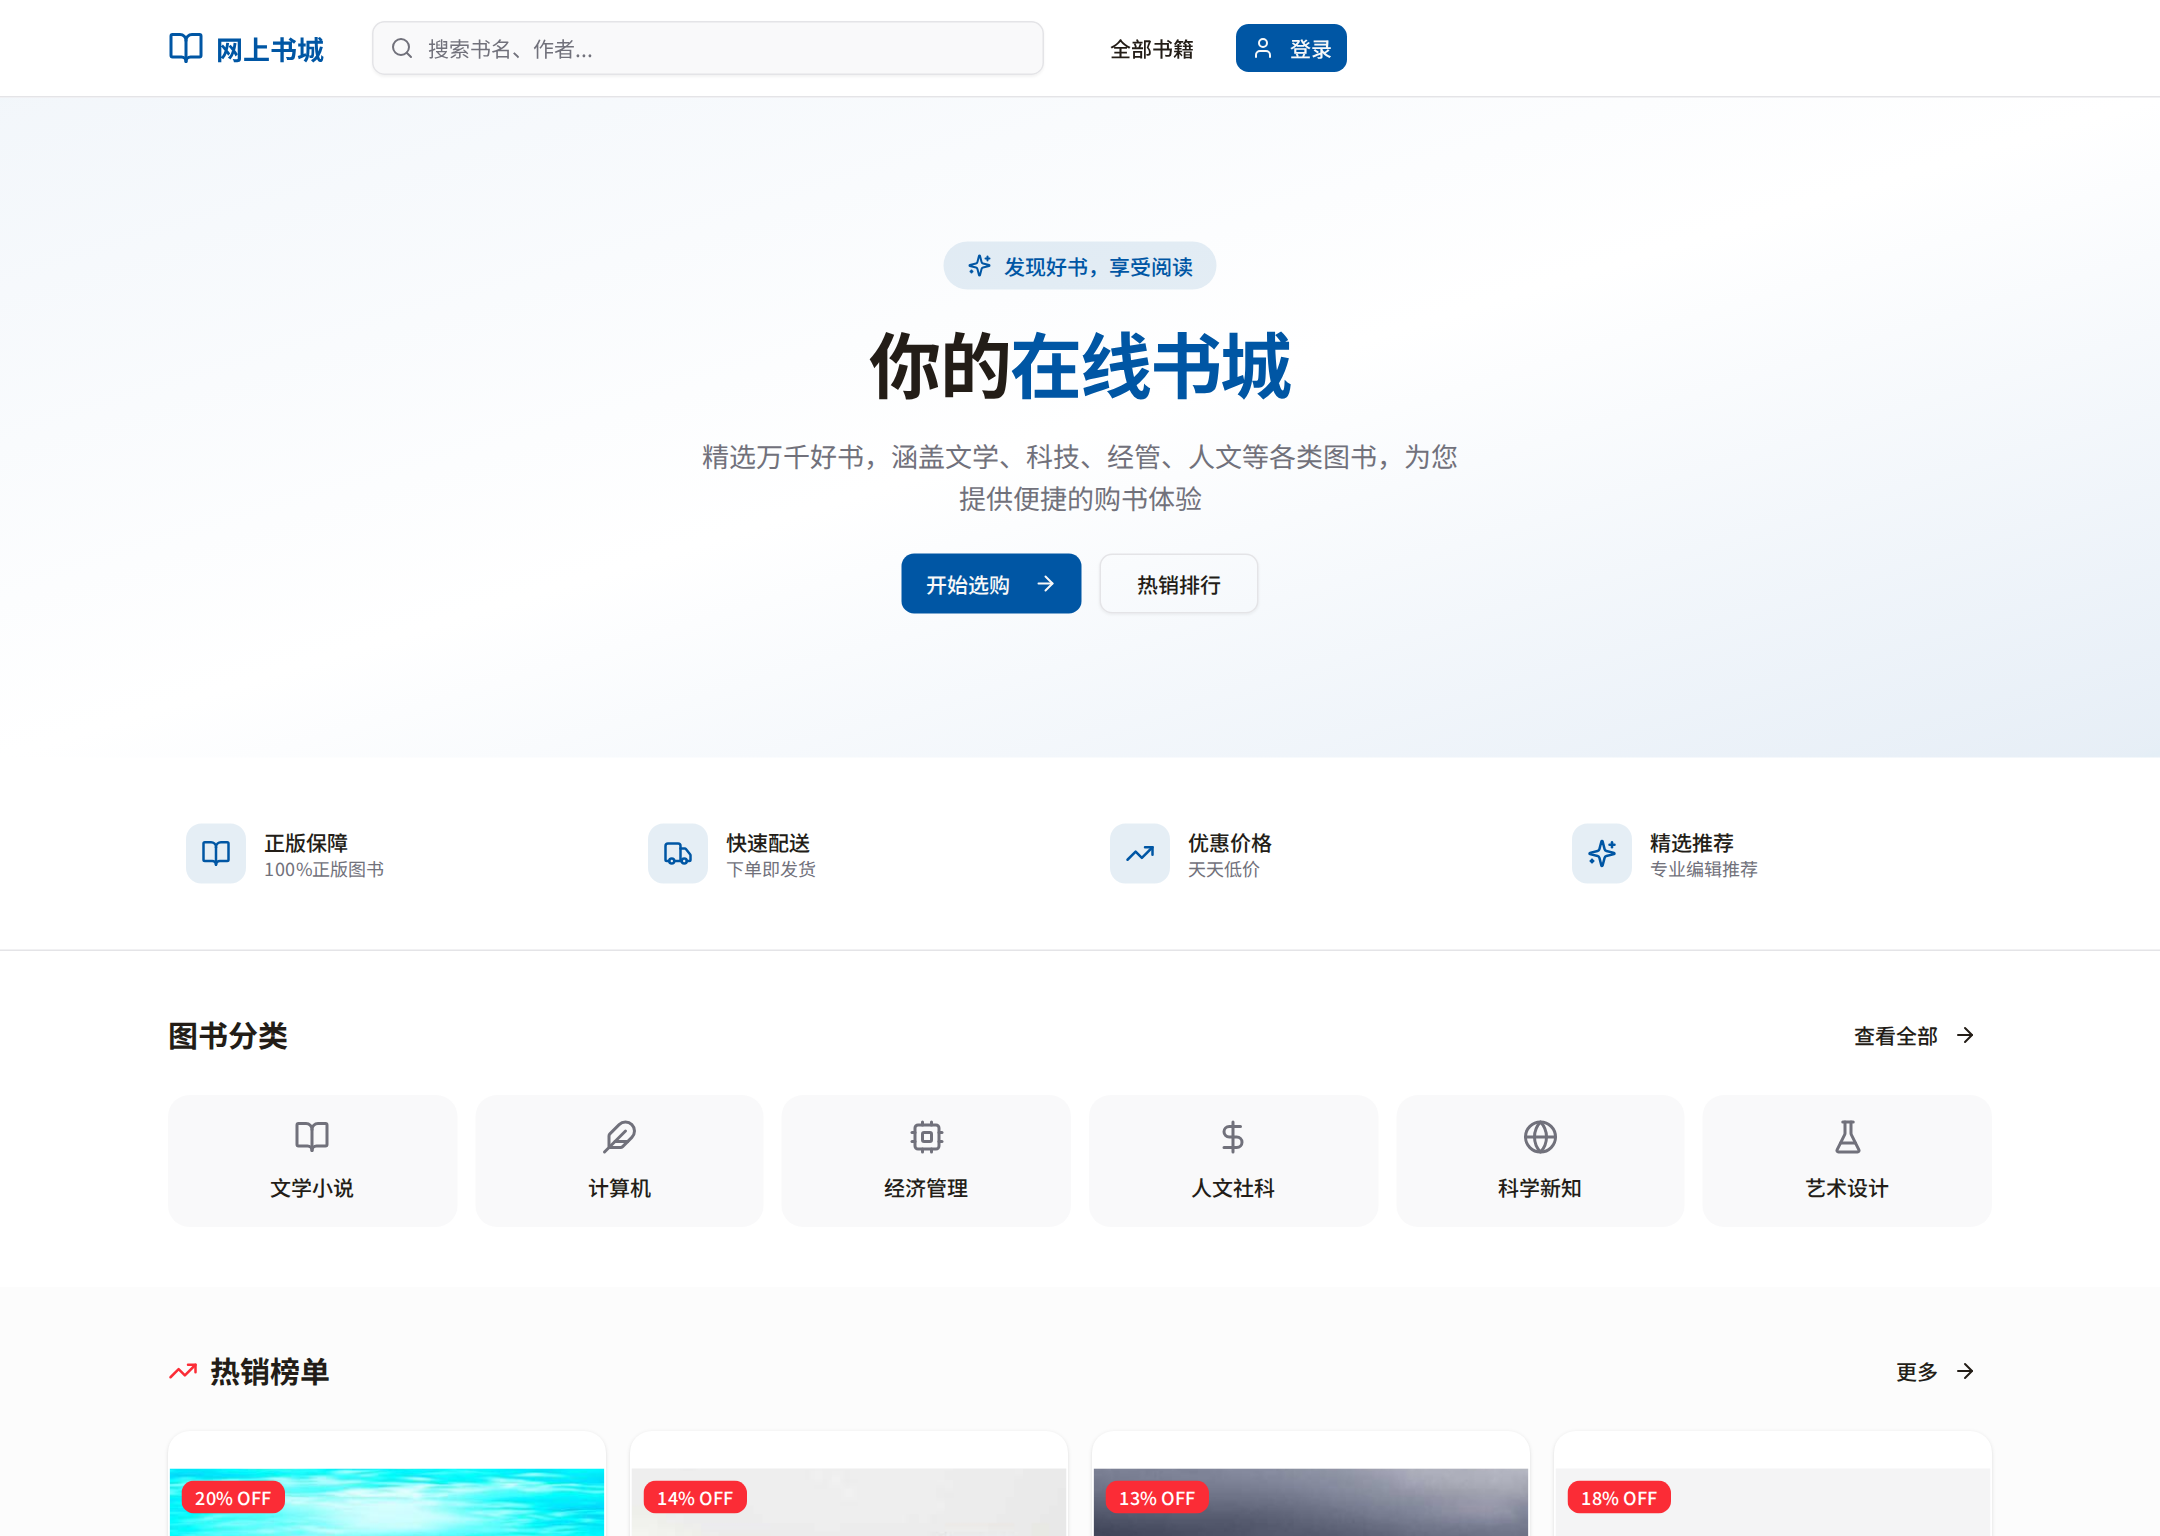
\includegraphics[width=0.92\textwidth]{screenshots/01-home.png}
  \caption{系统首页界面}
  \label{fig:home-page}
\end{figure}

% 单张界面图示例：购物车
\begin{figure}[H]
  \centering
  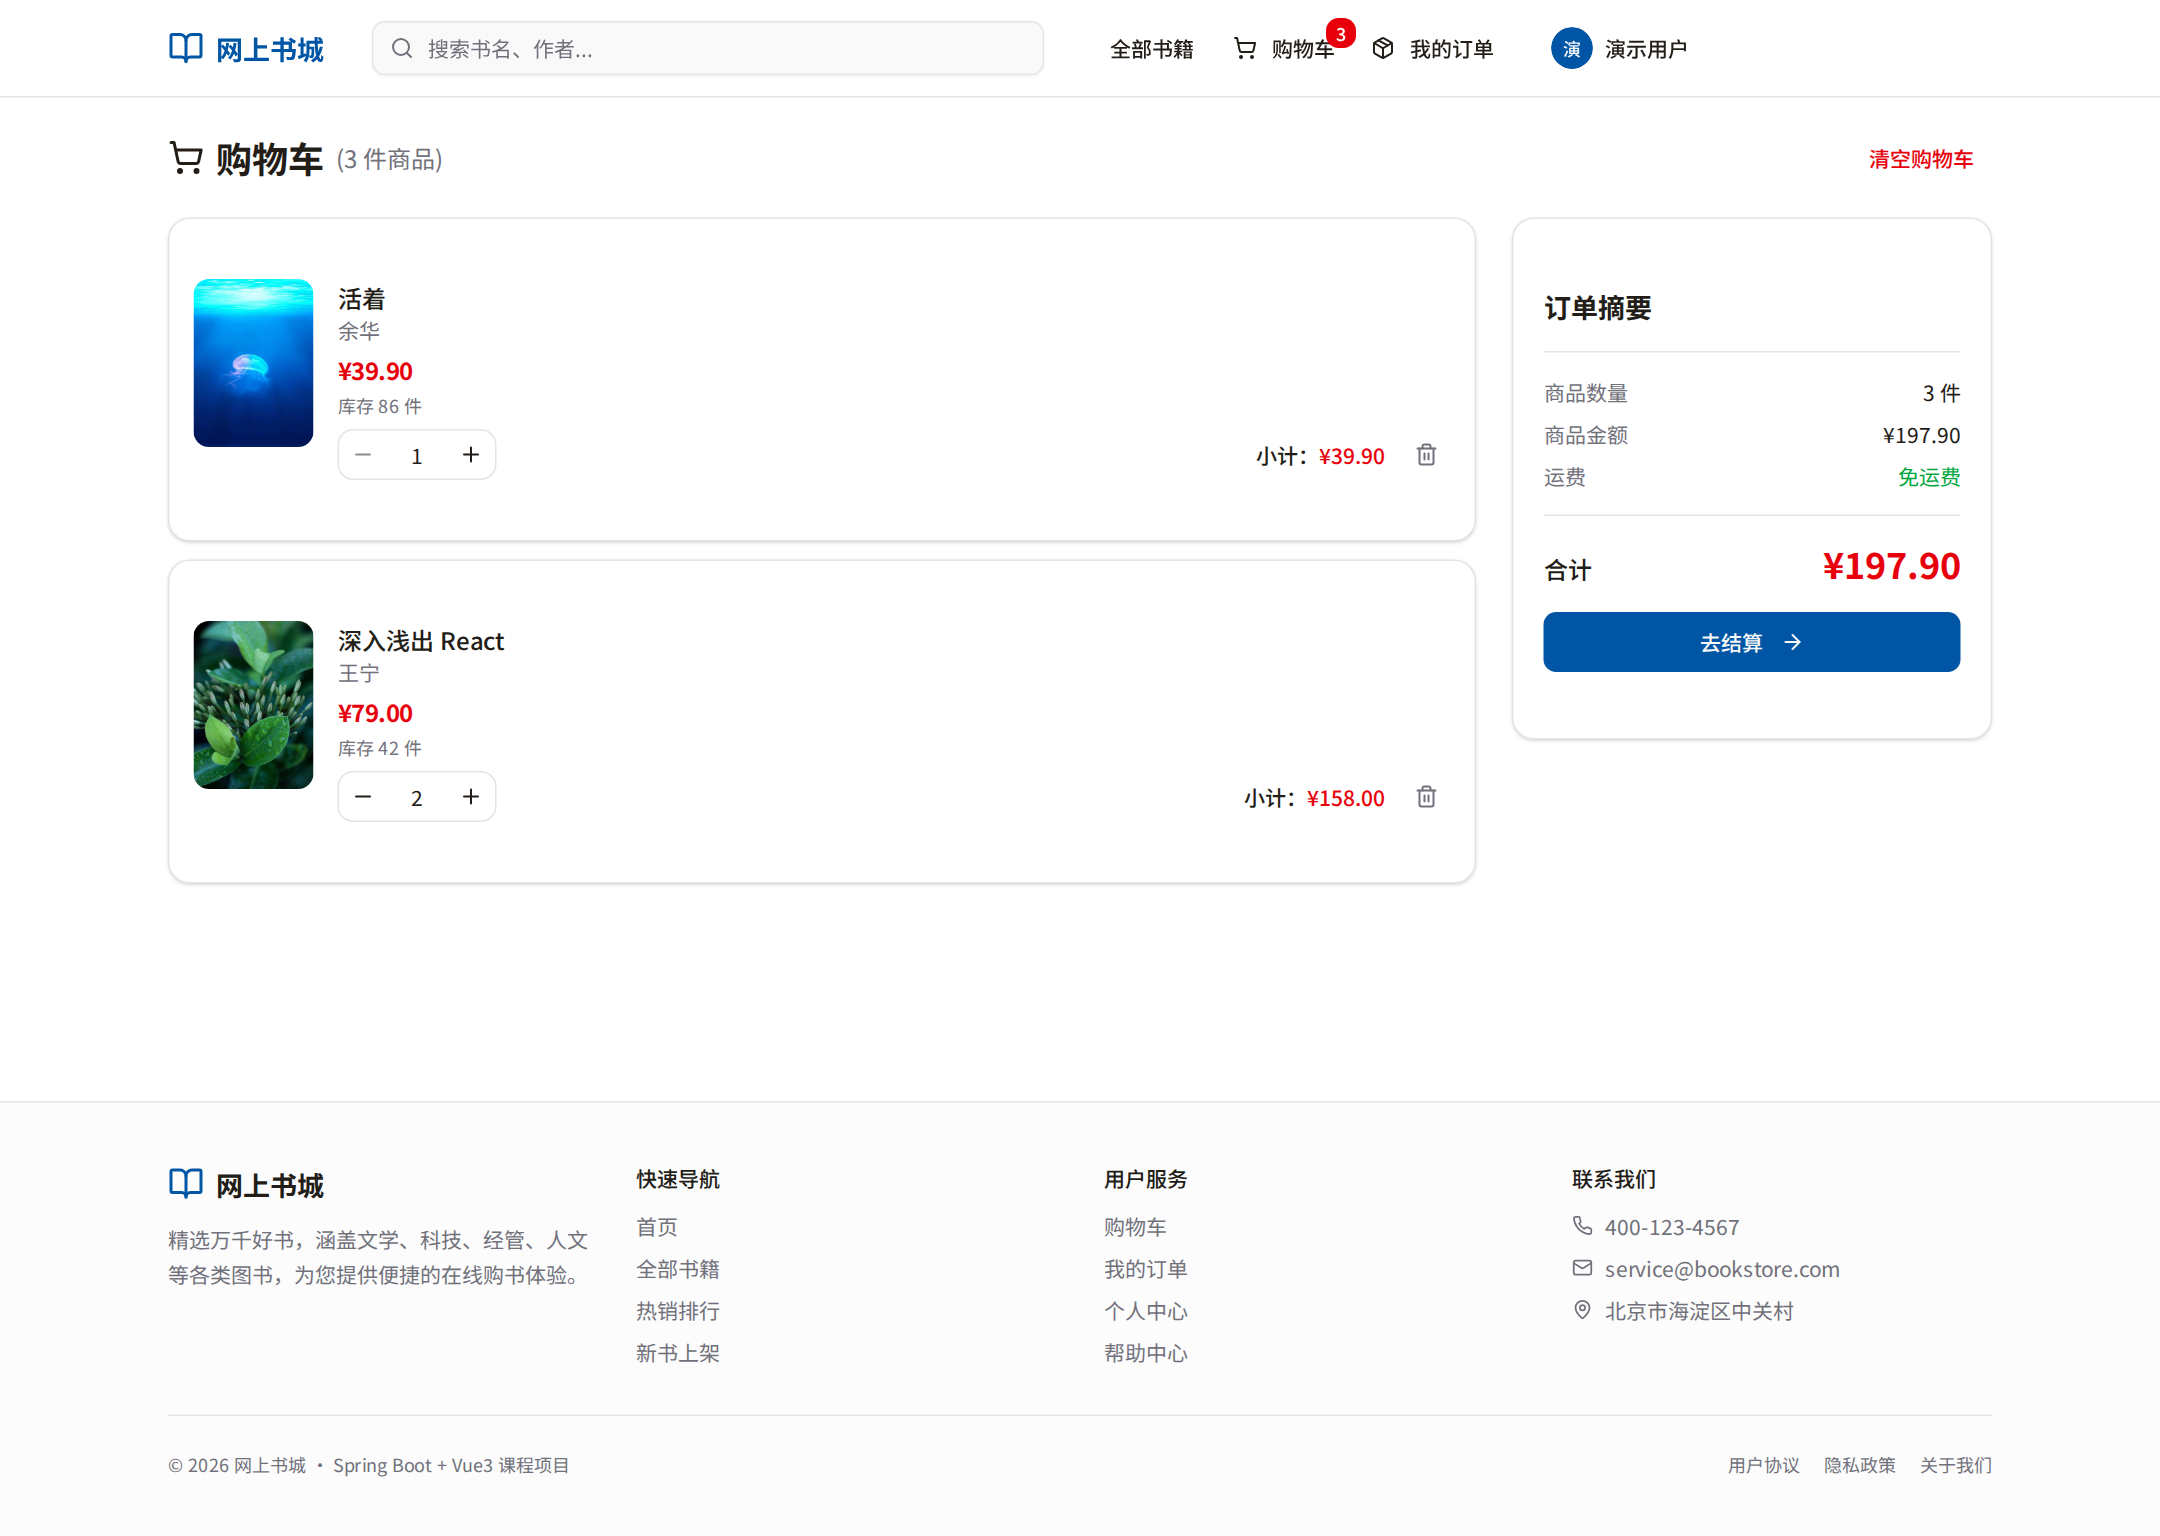
\includegraphics[width=0.92\textwidth]{screenshots/04-user-cart.png}
  \caption{购物车管理界面}
  \label{fig:user-cart}
\end{figure}

% 两张图并排：订单列表与订单详情
\begin{figure}[H]
  \centering
  \begin{subfigure}[t]{0.48\textwidth}
    \centering
    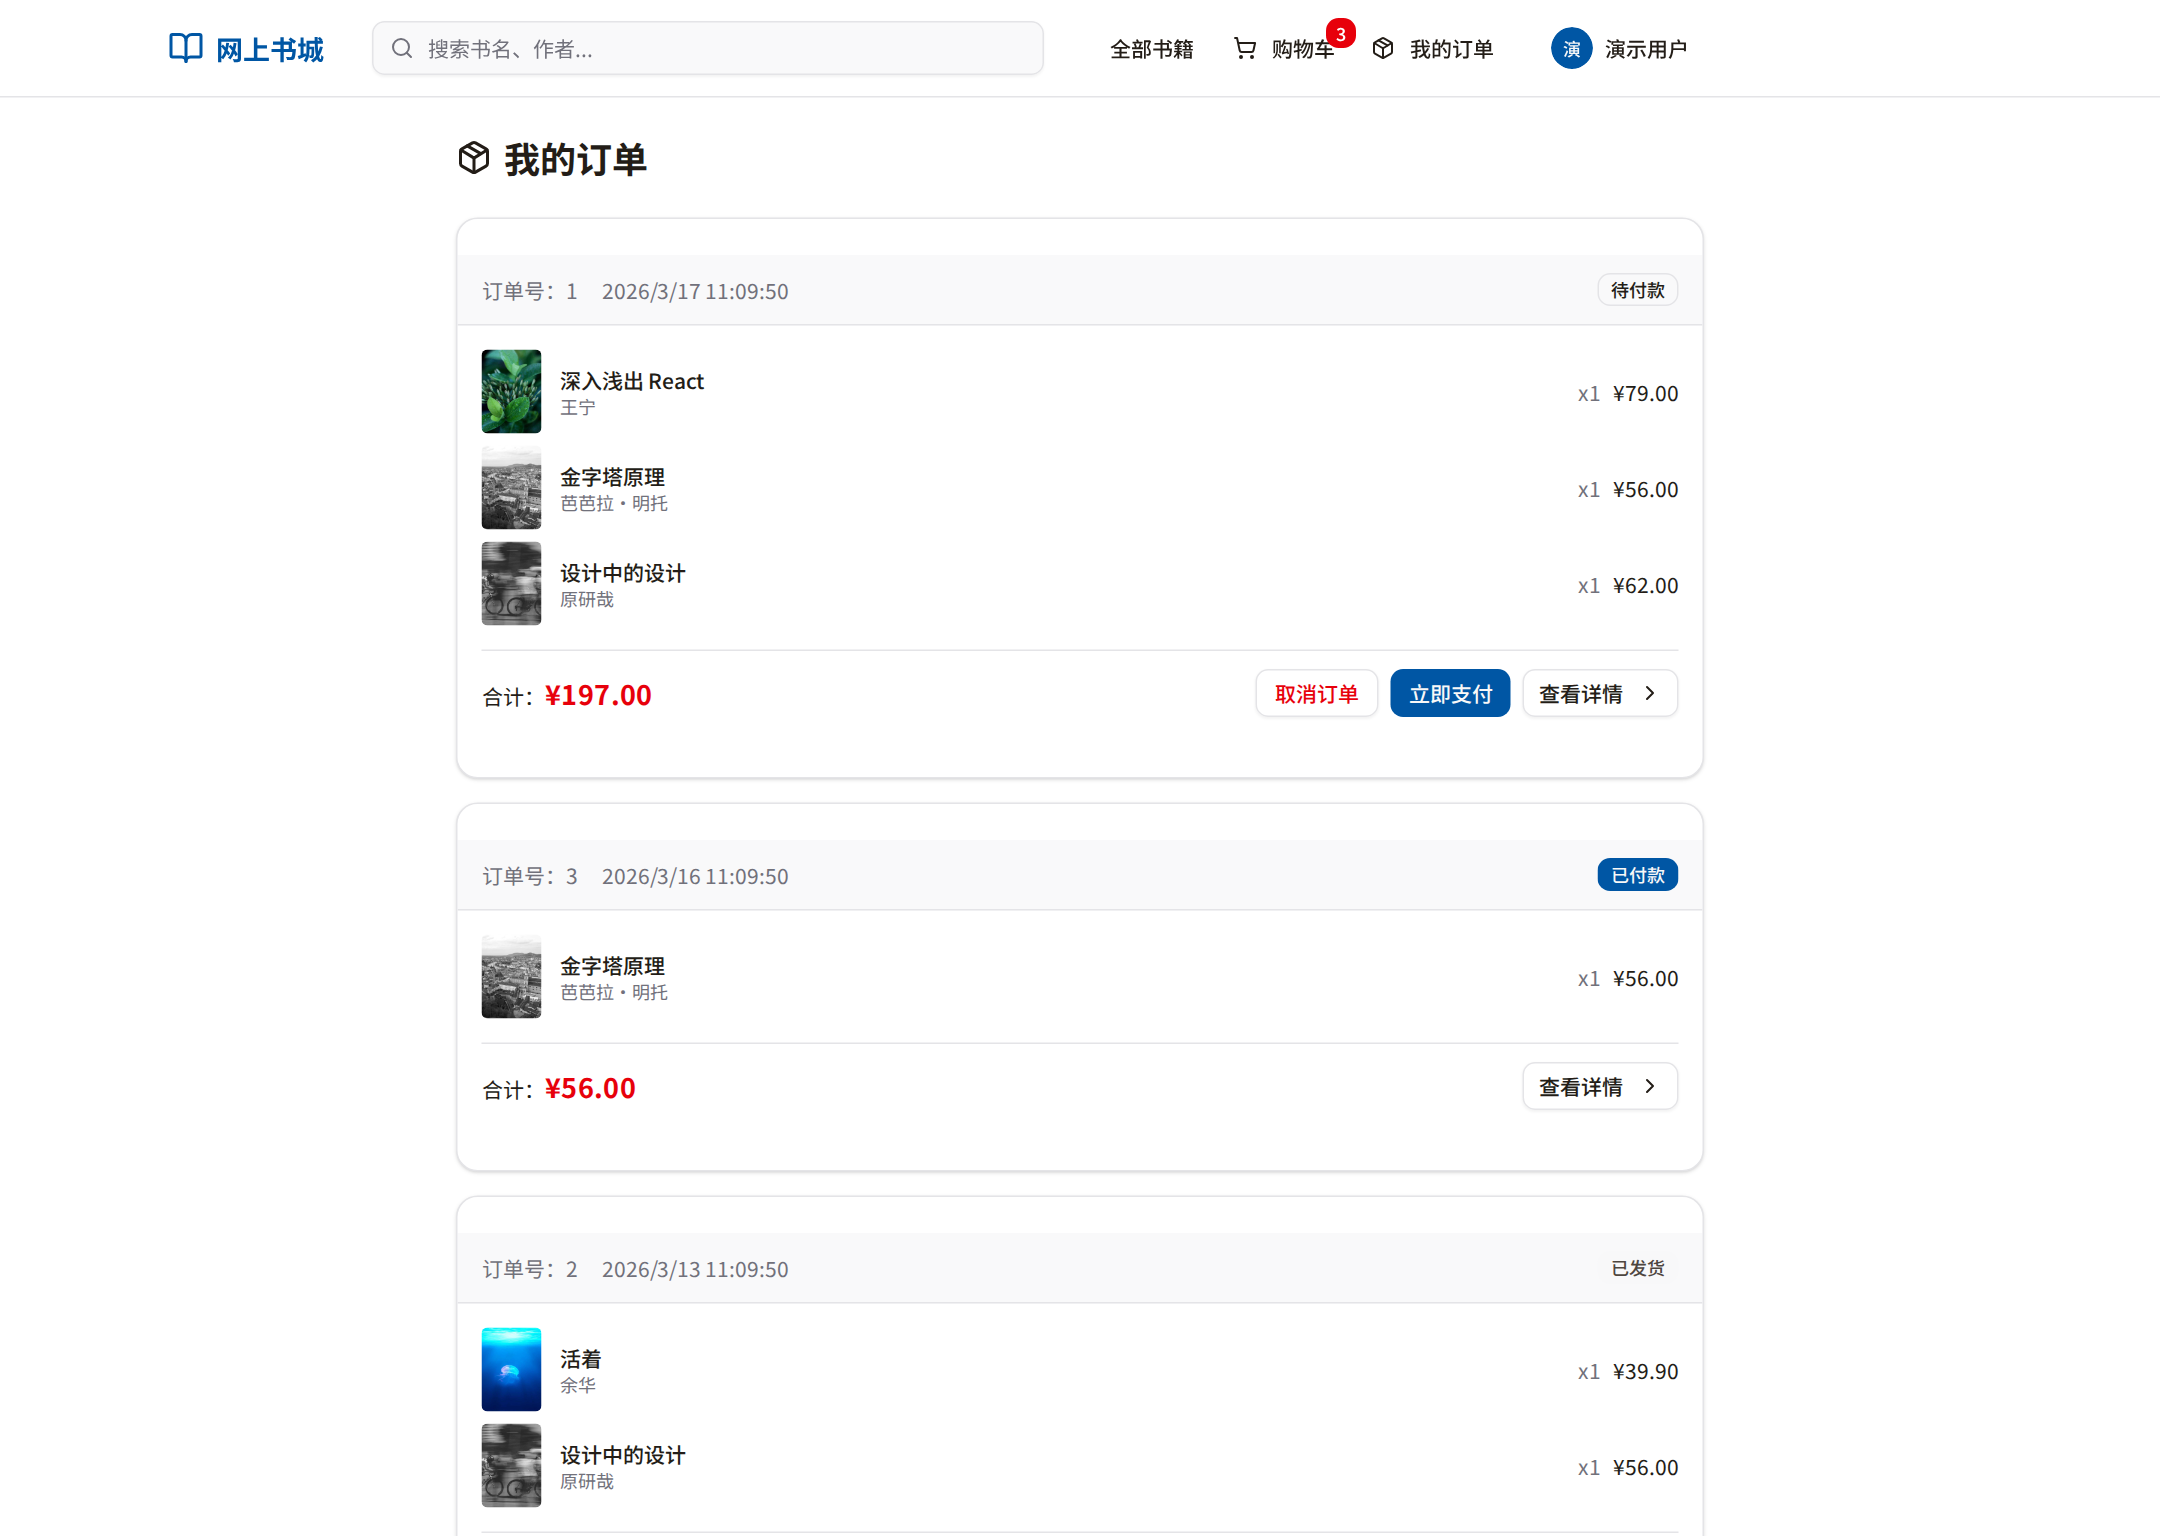
\includegraphics[width=\textwidth]{screenshots/06-user-orders.png}
    \caption{订单列表界面}
  \end{subfigure}
  \hfill
  \begin{subfigure}[t]{0.48\textwidth}
    \centering
    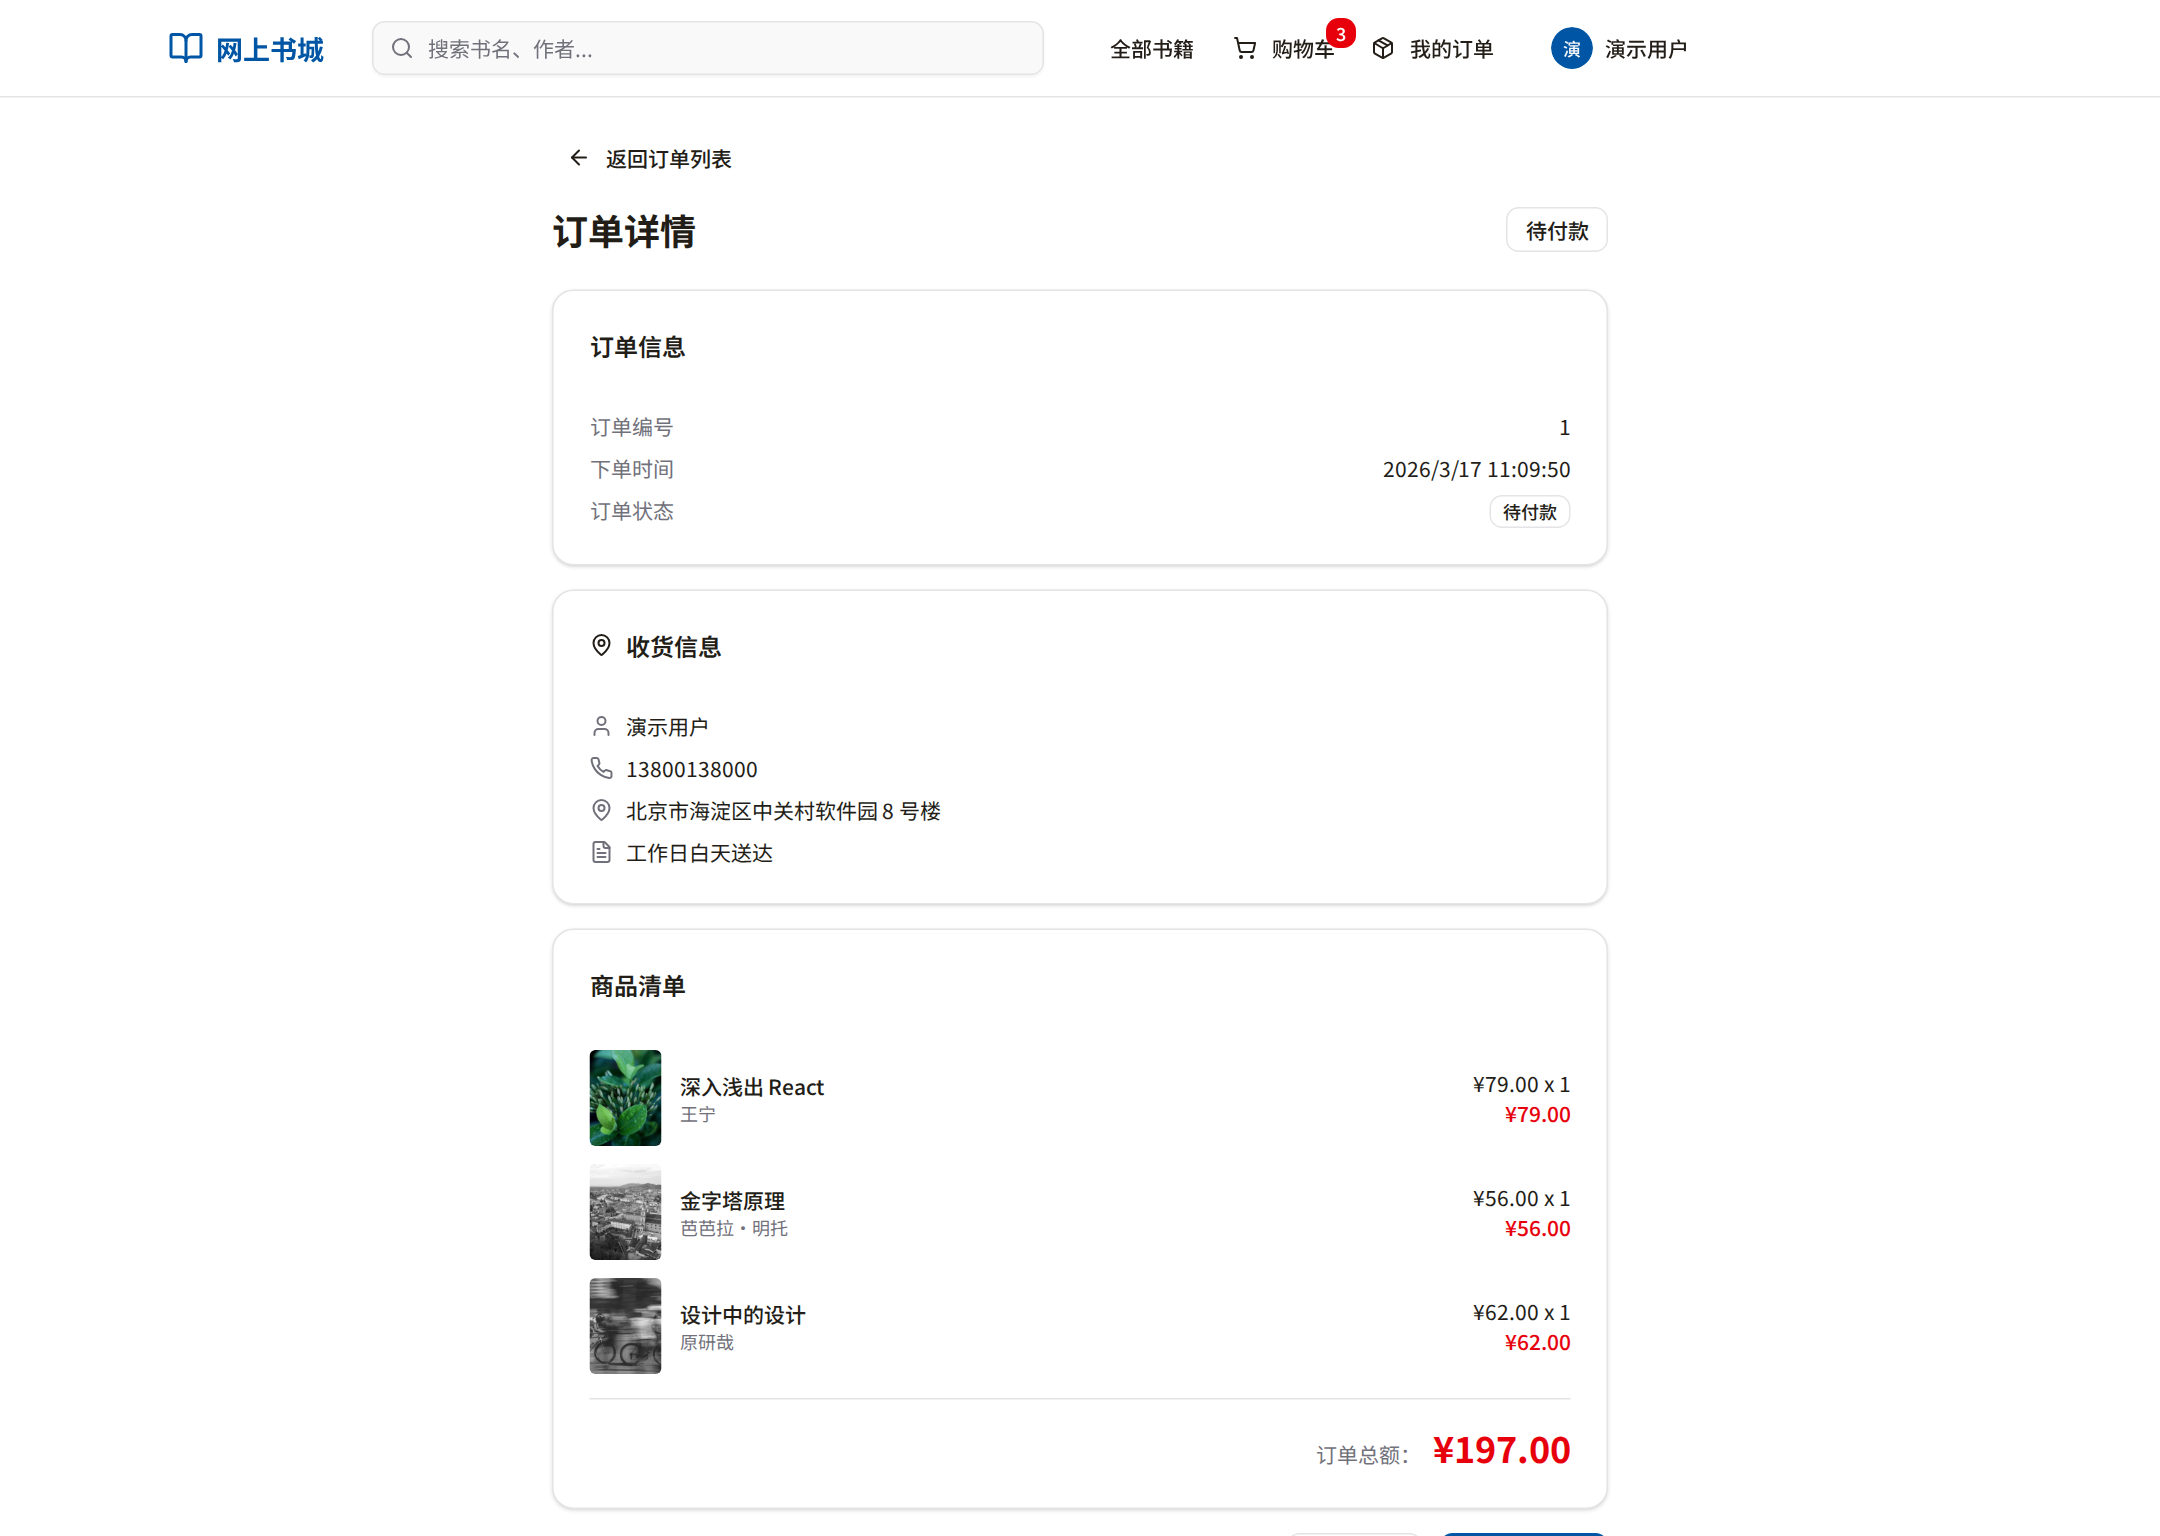
\includegraphics[width=\textwidth]{screenshots/07-user-order-detail.png}
    \caption{订单详情界面}
  \end{subfigure}
  \caption{用户订单功能界面展示}
  \label{fig:user-orders}
\end{figure}

% 两张图并排：后台书籍管理与分类管理
\begin{figure}[H]
  \centering
  \begin{subfigure}[t]{0.48\textwidth}
    \centering
    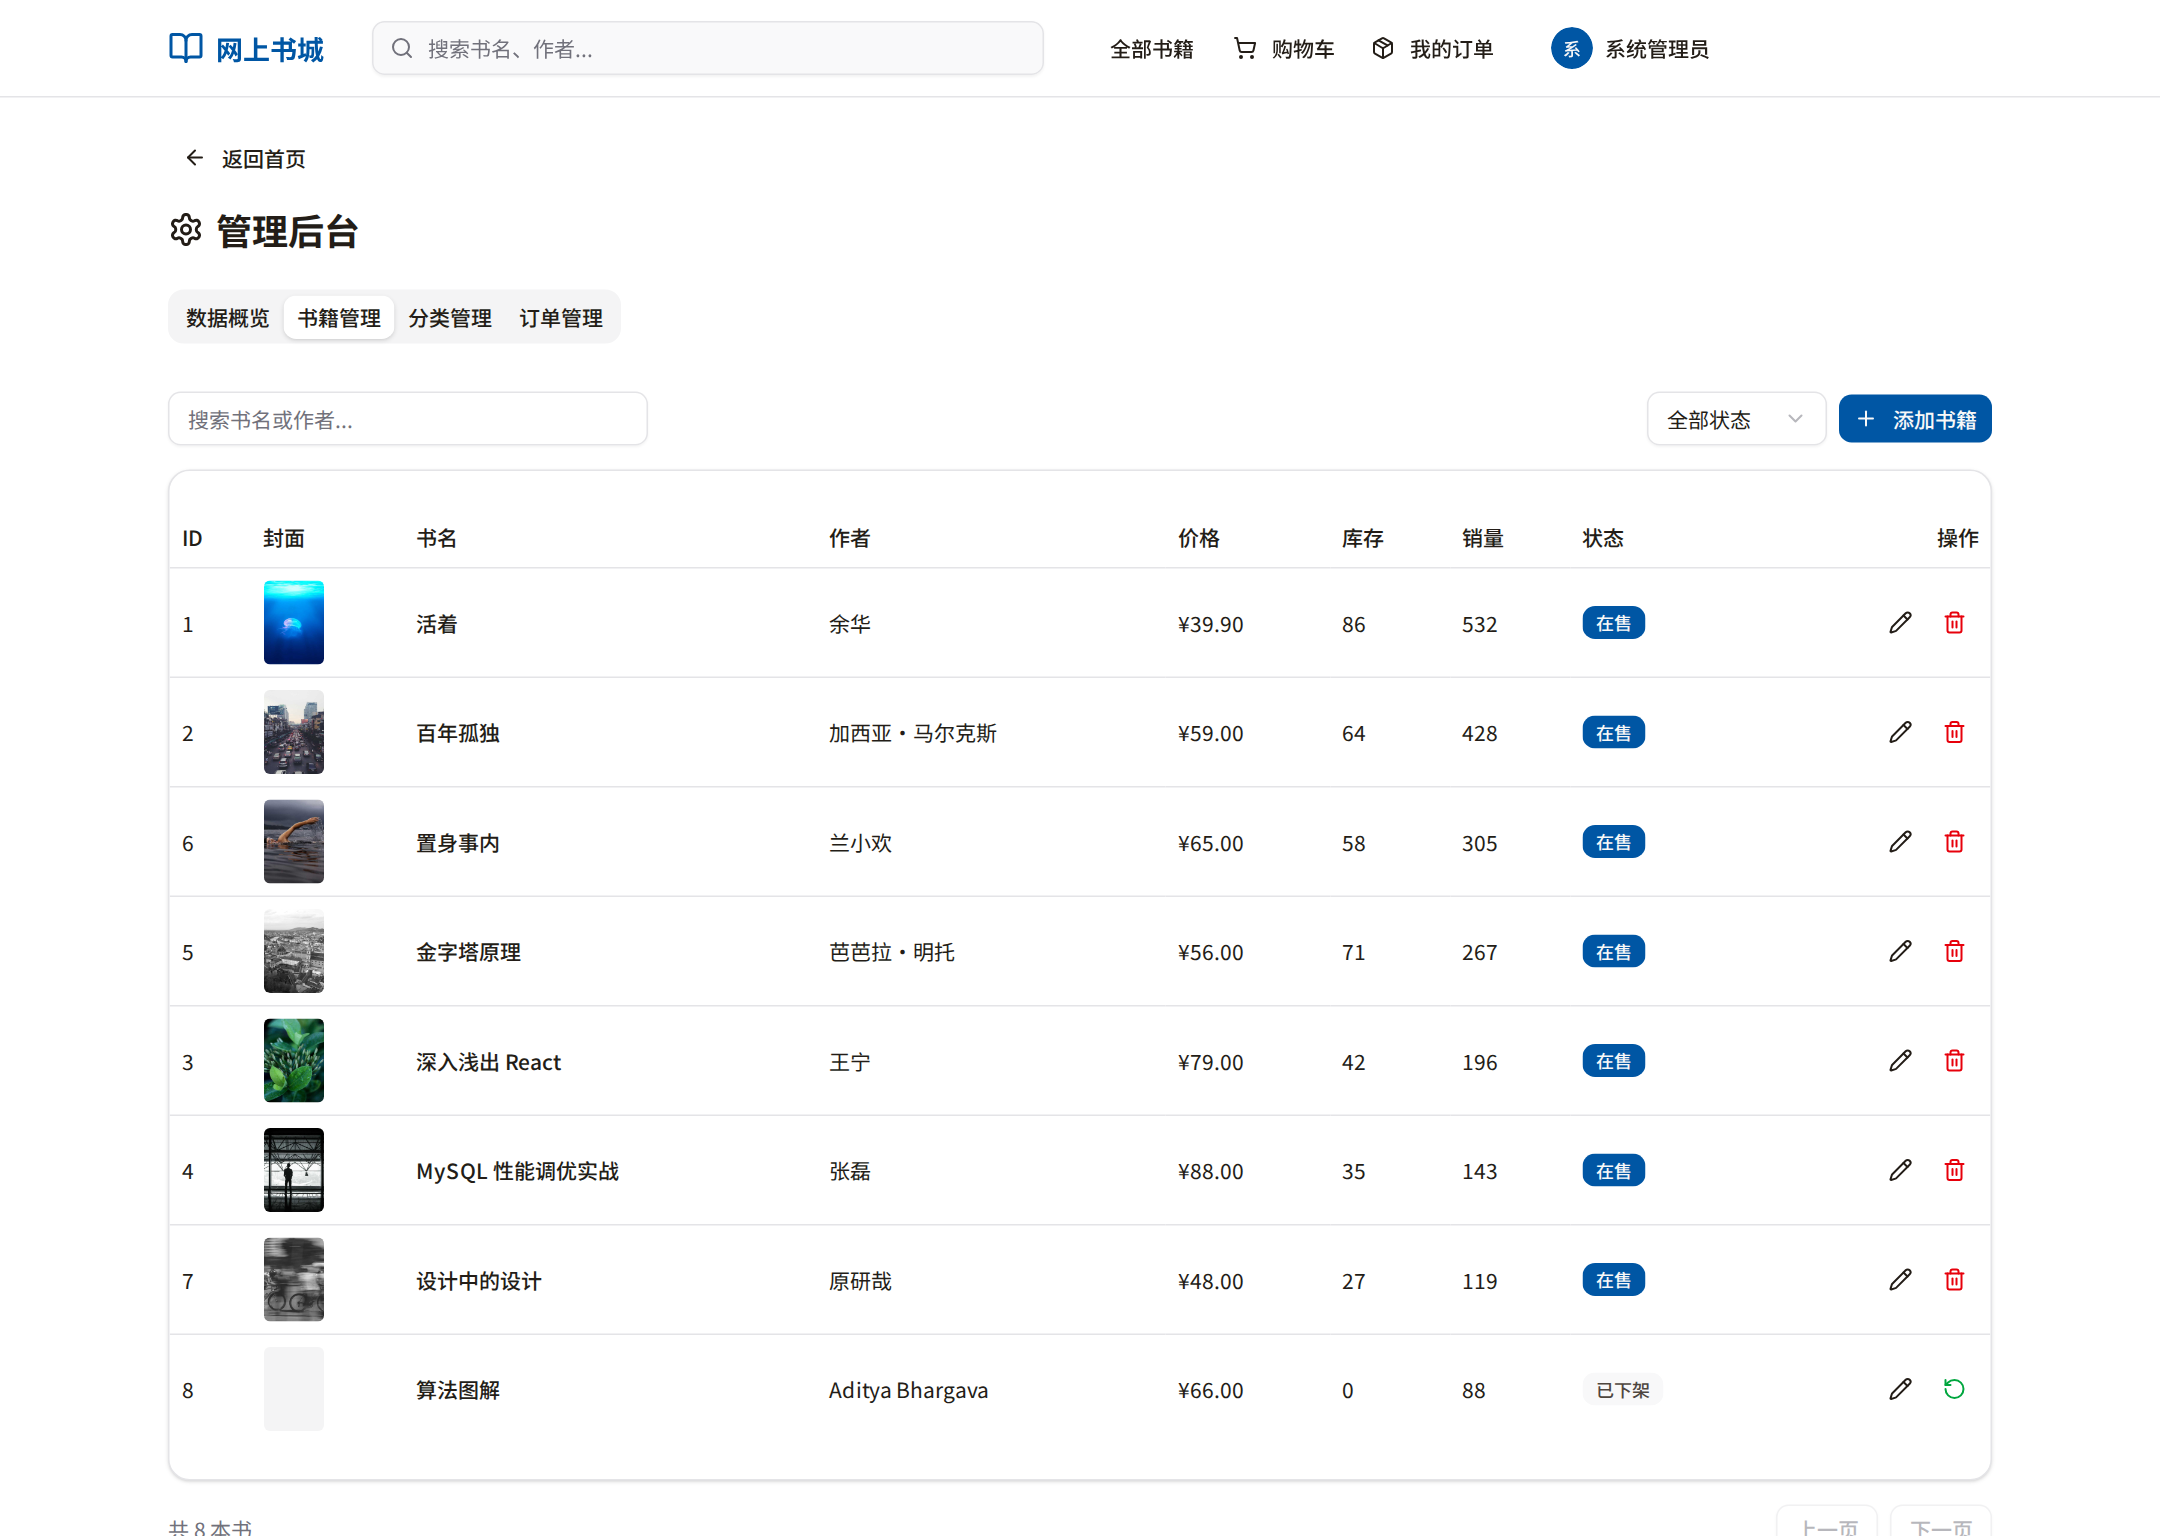
\includegraphics[width=\textwidth]{screenshots/10-admin-books.png}
    \caption{书籍管理界面}
  \end{subfigure}
  \hfill
  \begin{subfigure}[t]{0.48\textwidth}
    \centering
    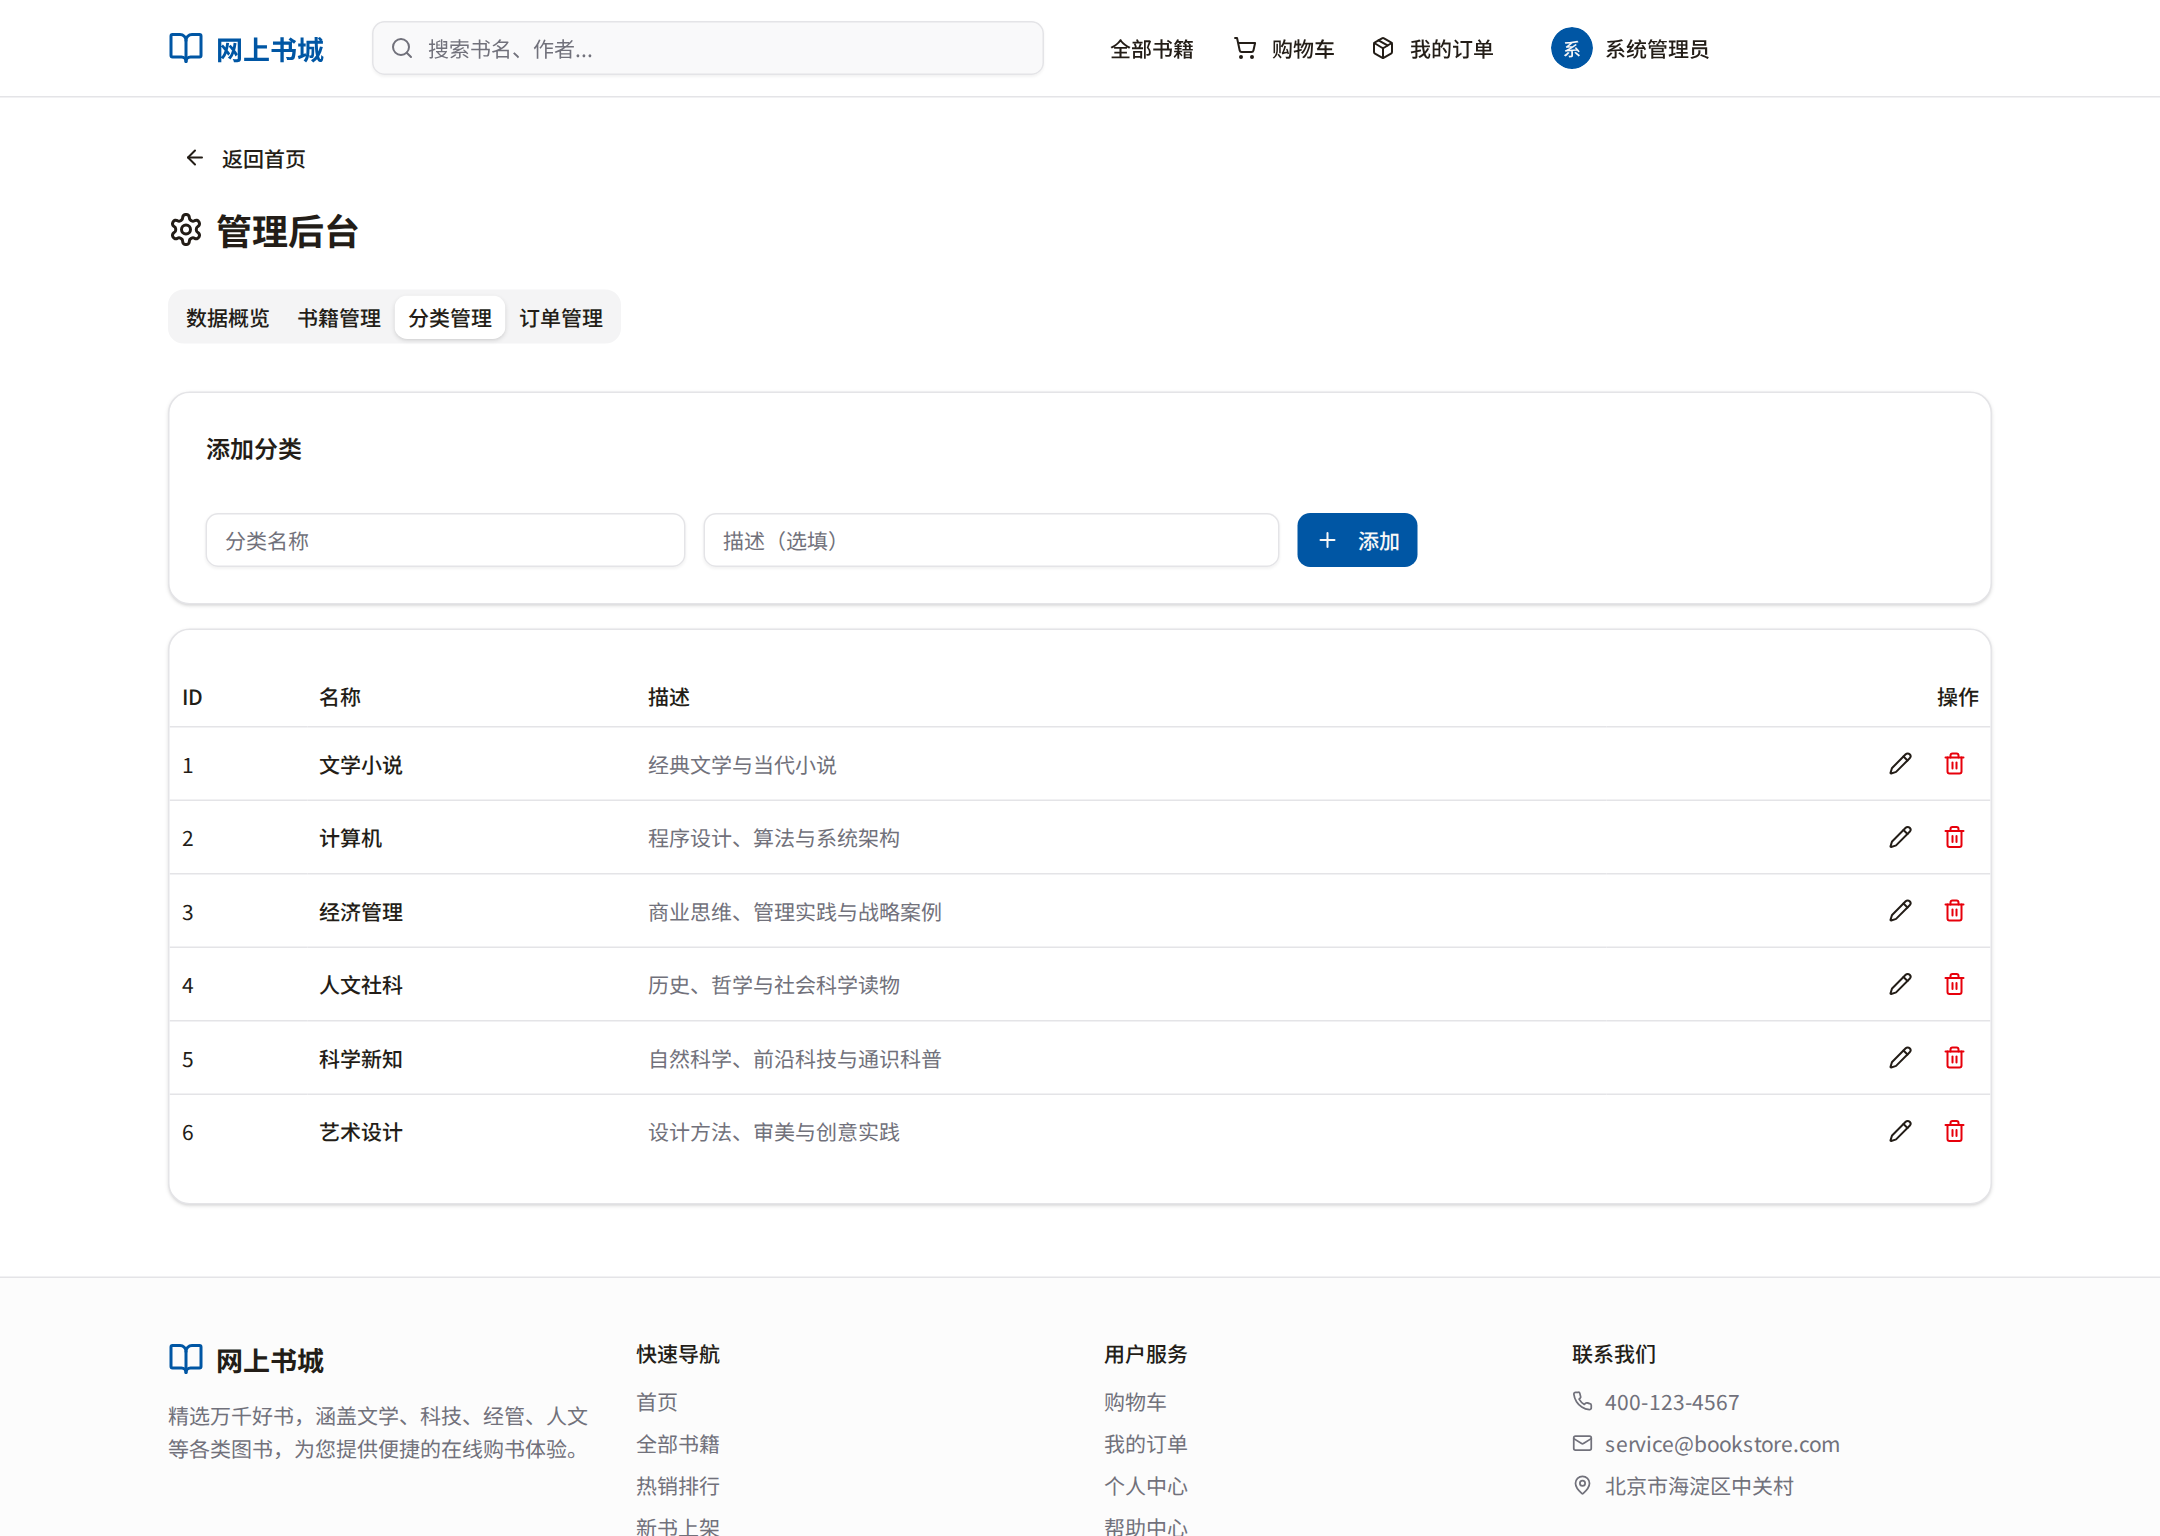
\includegraphics[width=\textwidth]{screenshots/11-admin-categories.png}
    \caption{分类管理界面}
  \end{subfigure}
  \caption{管理员端基础 CRUD 功能界面}
  \label{fig:admin-crud}
\end{figure}

% 结构图示例：页面关系图
\begin{figure}[H]
  \centering
  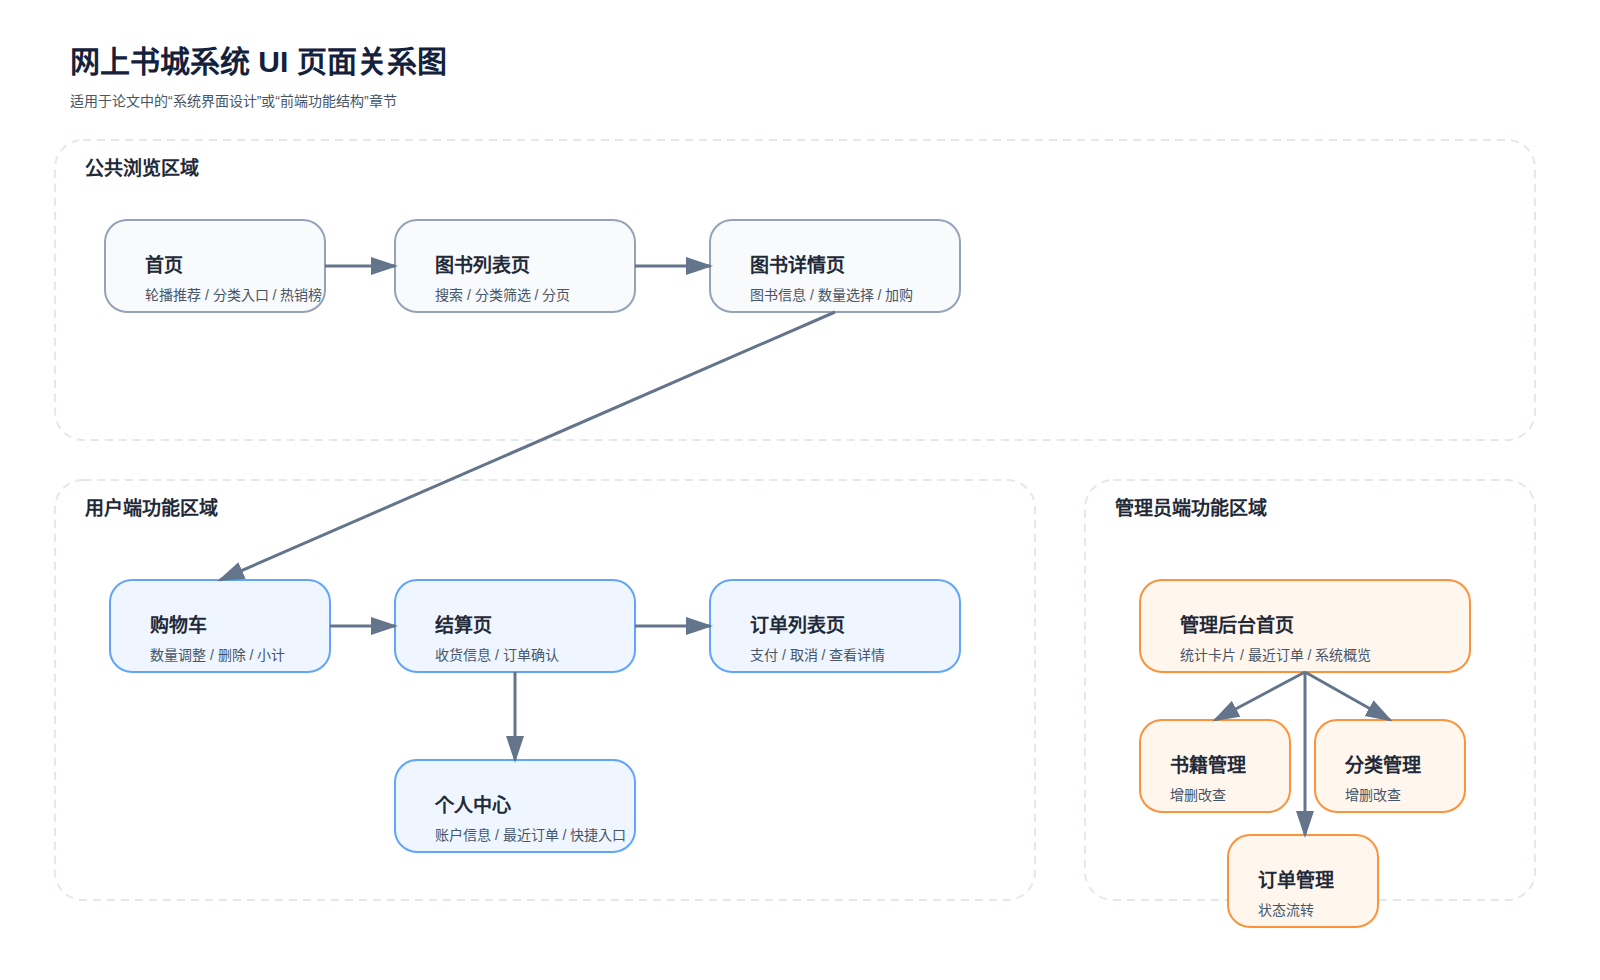
\includegraphics[width=\textwidth]{diagrams/ui_page_structure.png}
  \caption{系统 UI 页面关系图}
  \label{fig:ui-structure}
\end{figure}

% 结构图示例：角色功能模块图
\begin{figure}[H]
  \centering
  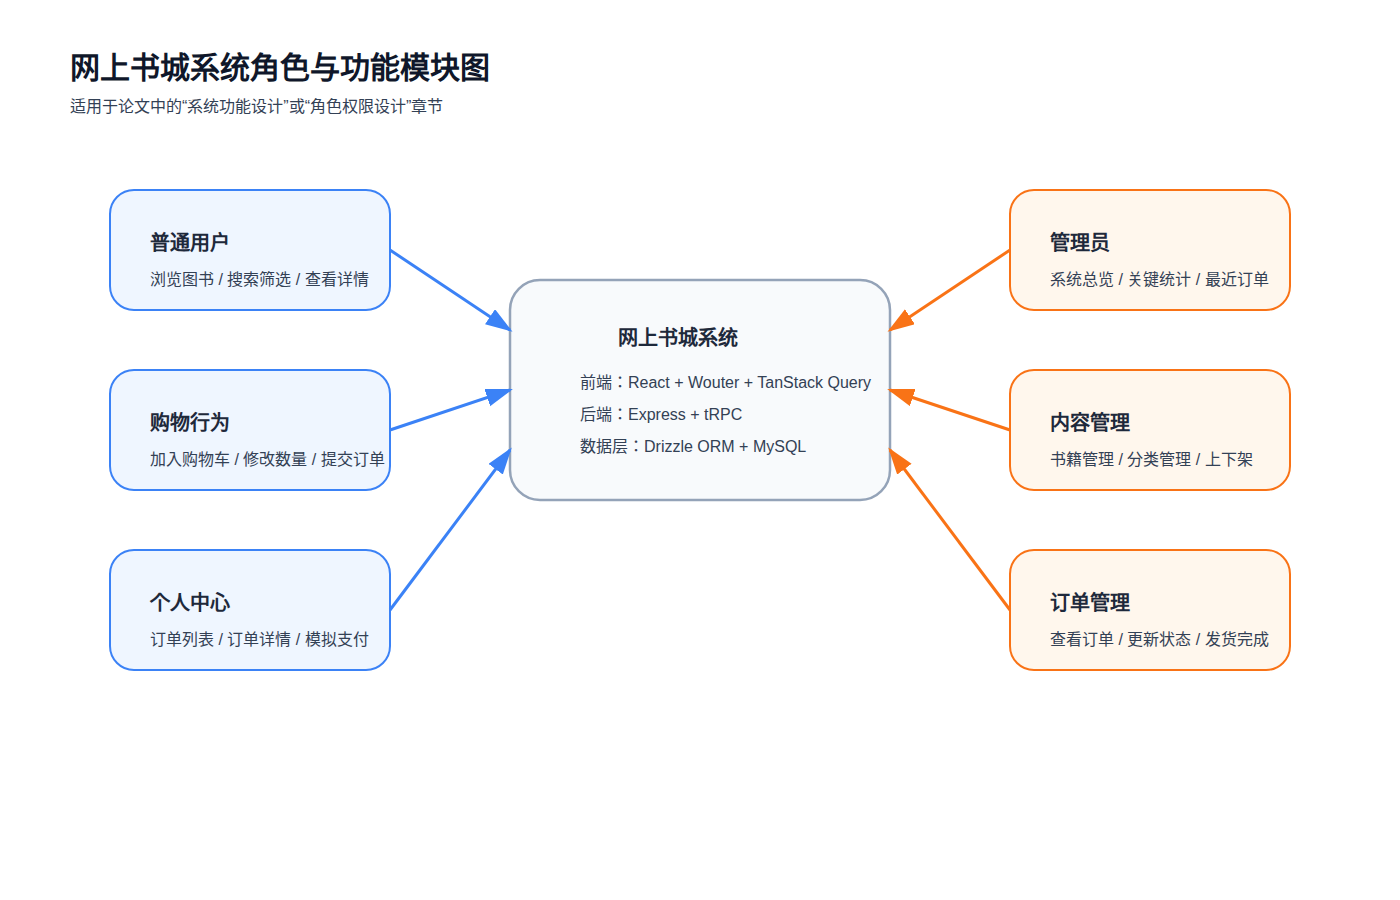
\includegraphics[width=0.95\textwidth]{diagrams/role_module_diagram.png}
  \caption{系统角色与功能模块图}
  \label{fig:role-module}
\end{figure}

% 流程图示例：用户购书流程图
\begin{figure}[H]
  \centering
  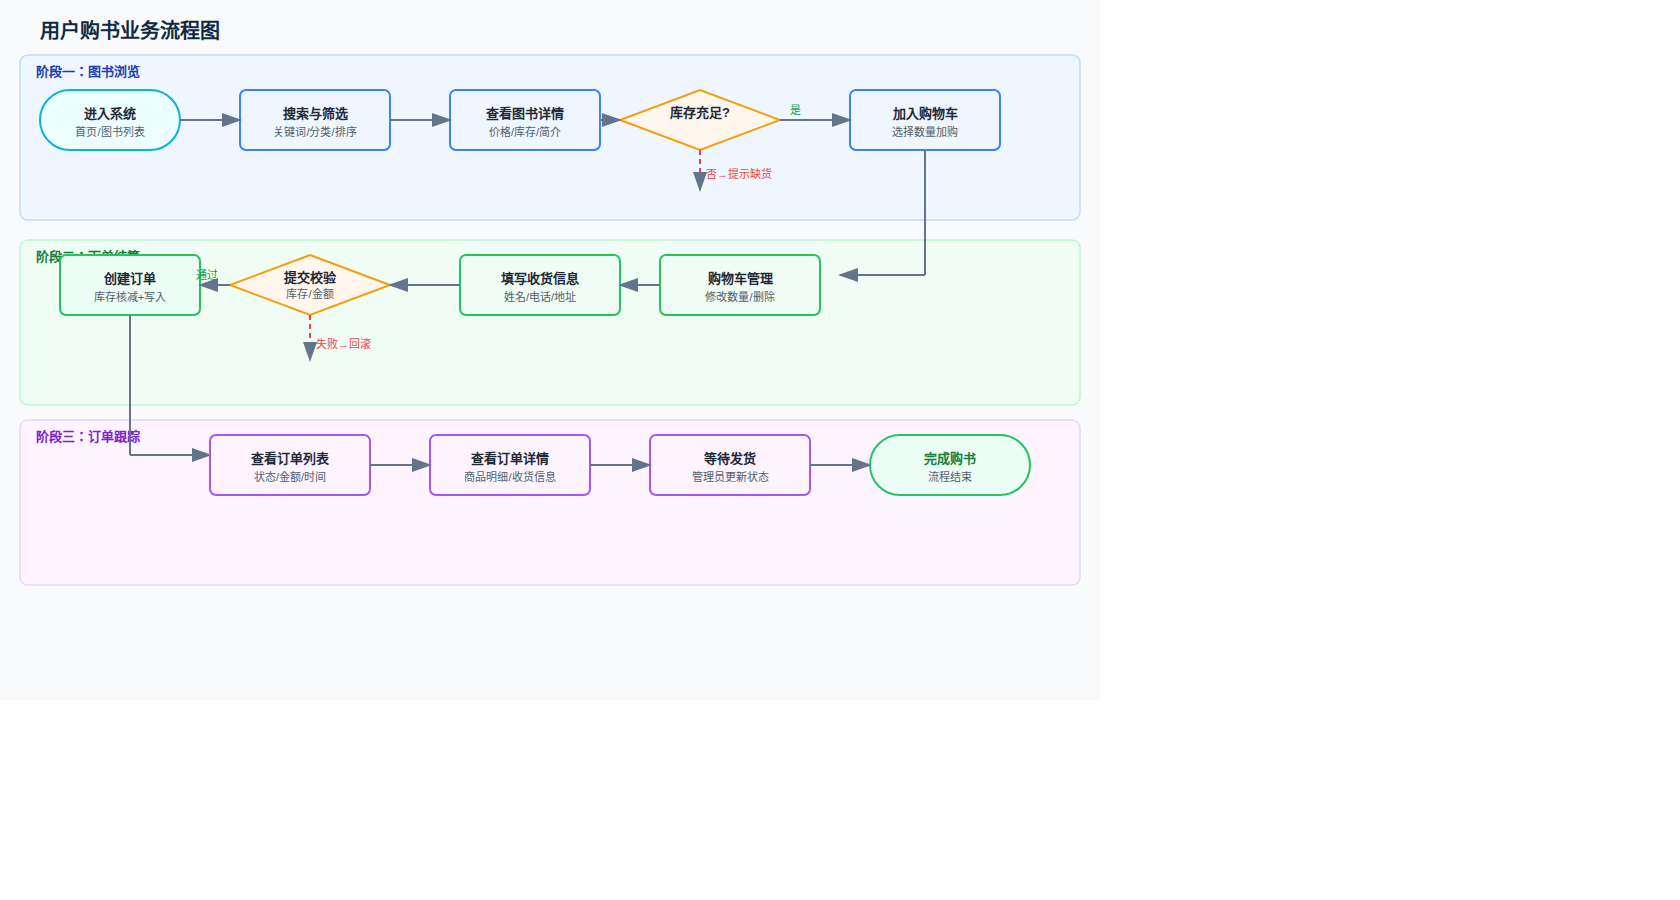
\includegraphics[width=\textwidth]{diagrams/user_purchase_flow.png}
  \caption{用户购书业务流程图}
  \label{fig:user-purchase-flow}
\end{figure}

% 流程图示例：管理员 CRUD 管理流程图
\begin{figure}[H]
  \centering
  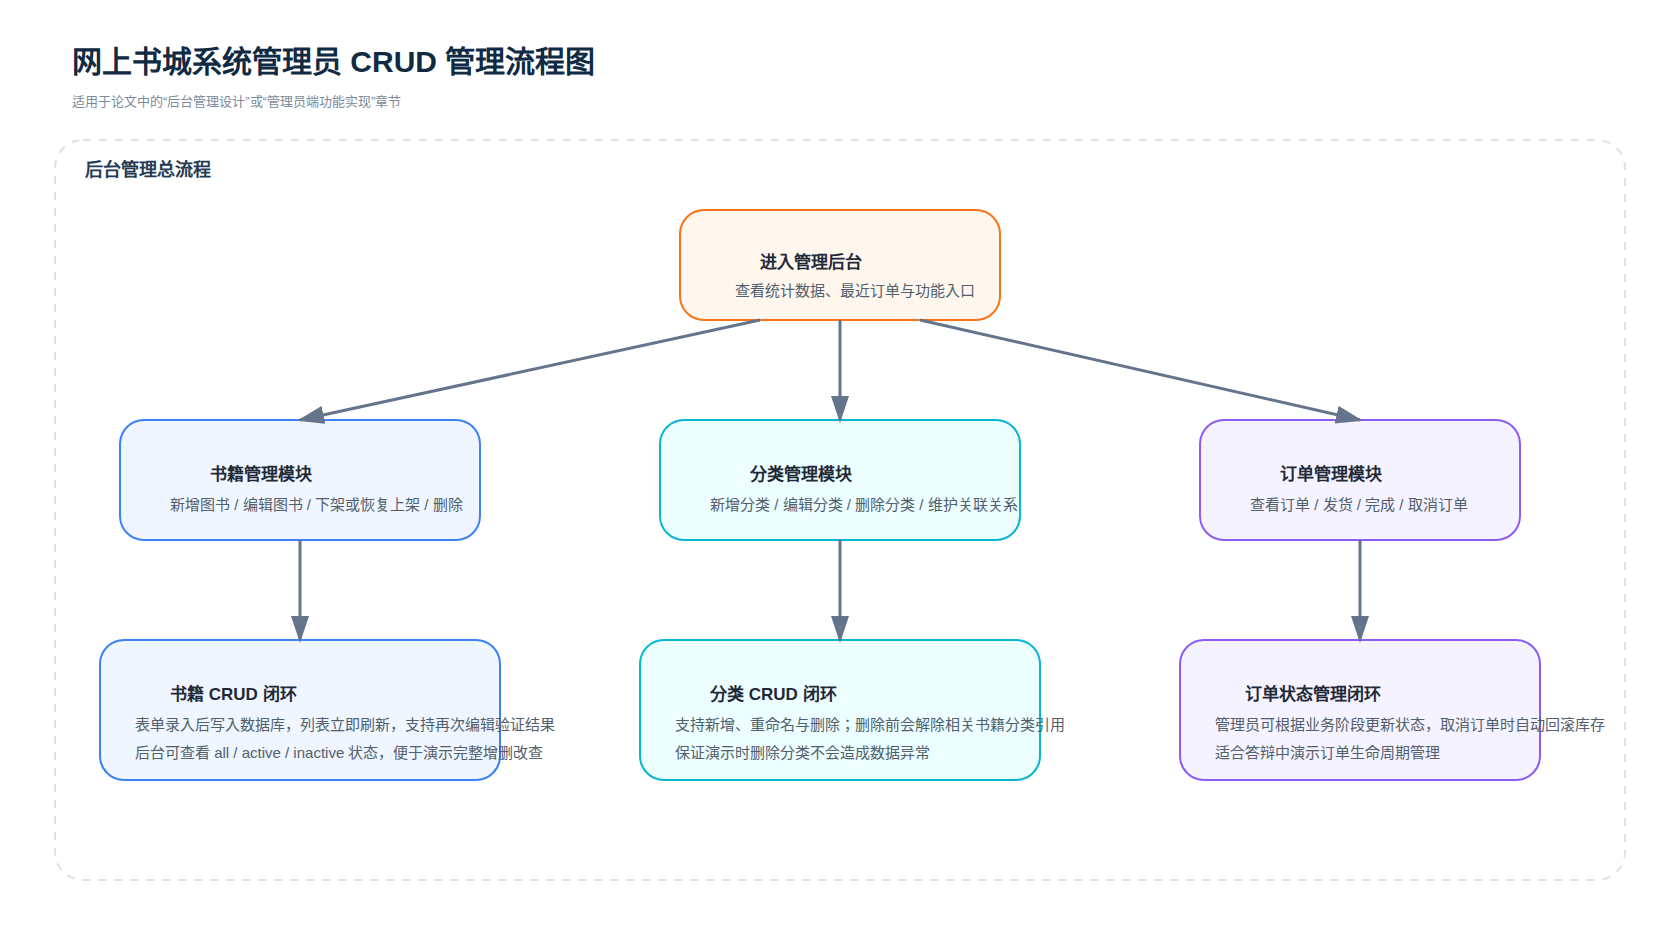
\includegraphics[width=\textwidth]{diagrams/admin_crud_flow.png}
  \caption{管理员 CRUD 管理流程图}
  \label{fig:admin-flow}
\end{figure}
